


\section{Results and Analysis}\label{sec:results}
\begin{figure*}[t!]
    \centering

    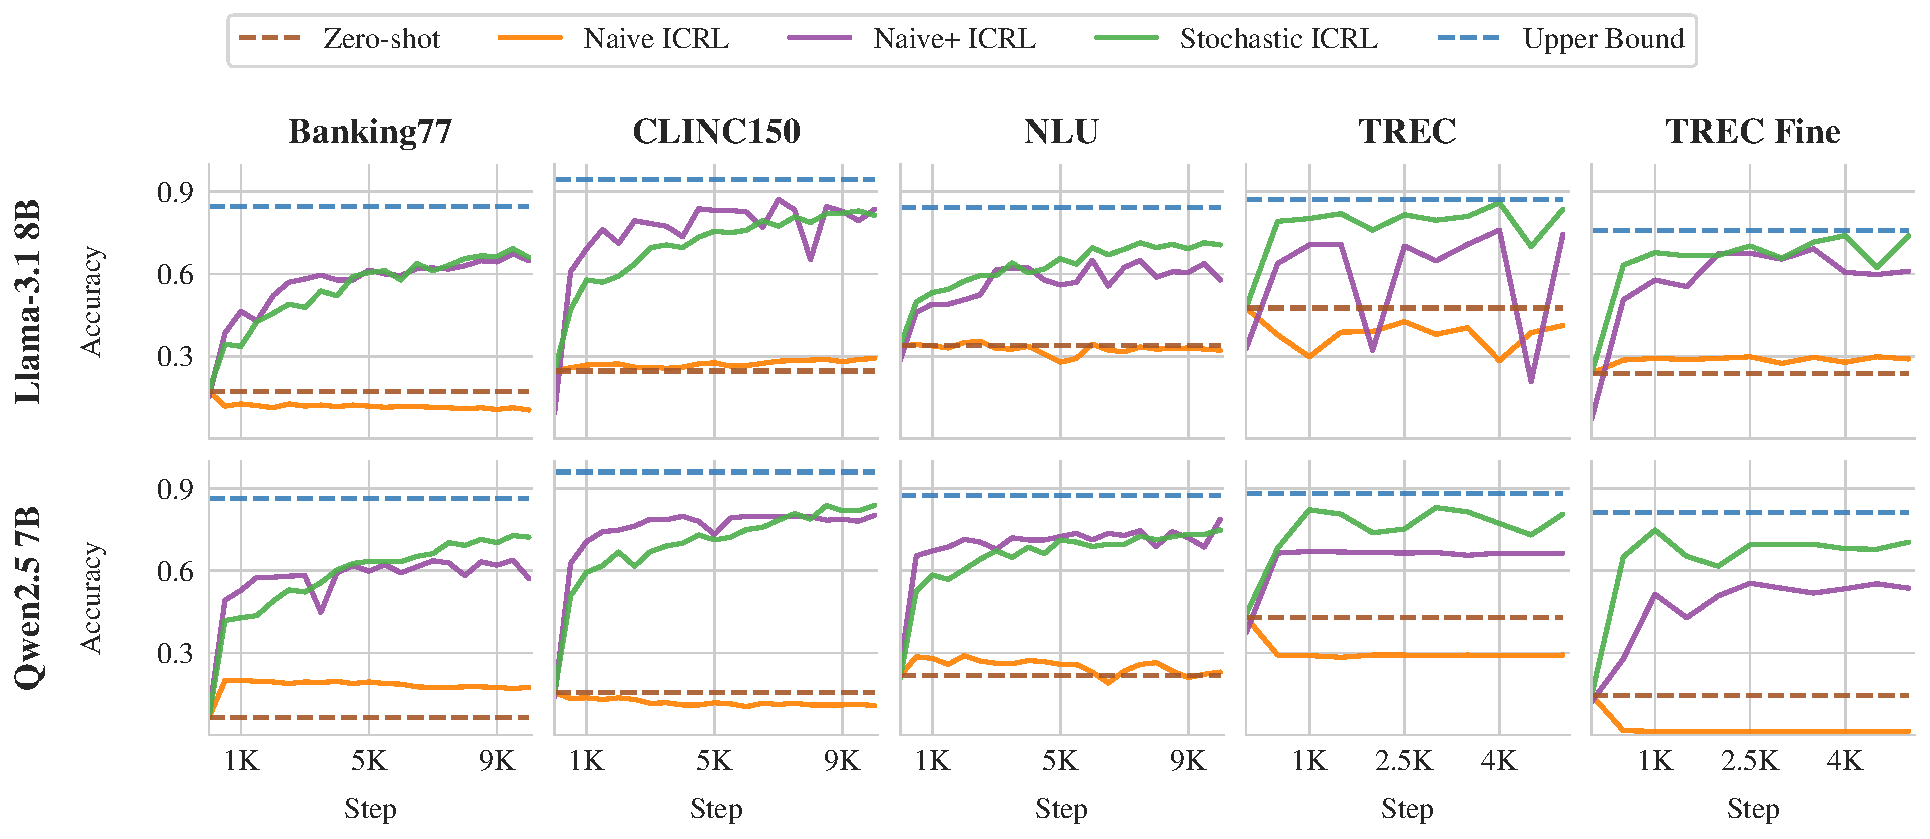
\includegraphics[width=1.0\textwidth]{figures/main_results/main_results.pdf}
    \caption{\textbf{Performance of ICRL.} \naiveshort, \naiveplusshort, and \expshort held-out test results for \llama and \qwen and all tasks. \naiveplusshort and \expshort consistently outperform zero-shot (i.e., first step) and \naiveshort, while also showing consistent trends of continual improvement as more data is observed. \autoref{tab:main_results} in \aautoref{sec:appendix:results} details start and end accuracies.}
    \label{fig:main_results}
\vspace{-15pt}
\end{figure*}

\autoref{fig:main_results} shows the test accuracies for \llama~3.1 8B and \qwen{2.5} 7B. 
As an upper bound to in-context learning, we also show the performance of an oracle with access to the gold labels for the maximum number of in-context examples that the model can fit. Unless specified otherwise, we use $p_{keep} = 0.1$ and sampling temperature $T = 1.0$ for \expshort and zero-shot, $T = 1.0$ for \naiveshort, and $T = 2.0$ for \naiveplusshort. We choose the best parameters for each ICRL method and include our analysis in \aautoref{appendix:icrl}.





\paragraph{LLMs Learn In-Context From Their Own Predictions and Rewards} 
Both \naiveplusshort and \expshort effectively learn in all tasks and for both models, showing significant improvements over zero-shot. 
\naiveplusshort and \expshort improve over the zero-shot  accuracies by between 28.6--74.4\% for \llama, and 29.2--68.4\% for \qwen. 
In general, accuracies approach the supervised performance in many settings, demonstrating the strong bandit ICRL capabilities of \llama and \qwen. 
Performance also grows monotonically over time, especially with \expshort,  suggesting further gains with more data. This trend is most evident in the most challenging datasets (\banking, \clinic, \nlu), where high label counts demand more exploration to map inputs to outputs.











\paragraph{Reward Signals Are Crucial, but Mistakes Remain Challenging}

\begin{wrapfigure}{r}{0.5\textwidth}  %
    \centering
    \vspace{-15pt}
    \subfloat{
        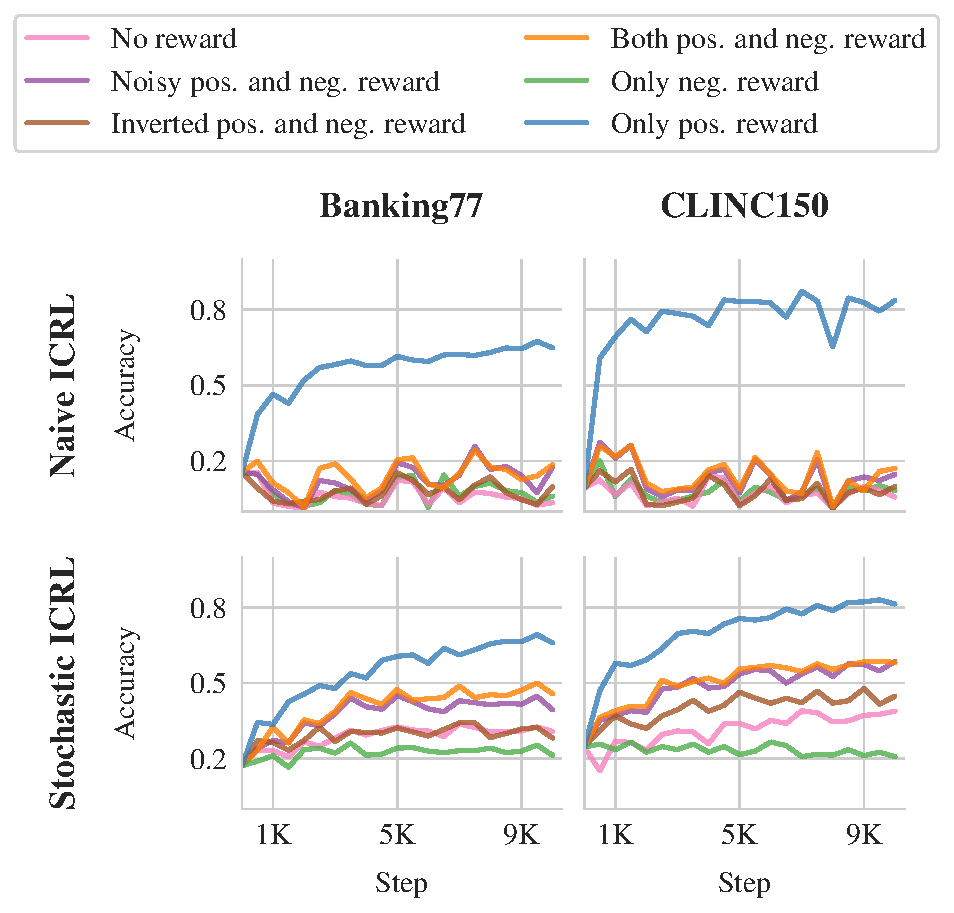
\includegraphics[width=0.48\textwidth]{figures/ablations/ablations_results_no_regret.pdf}
    }    
    \vspace{-5pt}\caption{\textbf{Reward ablations.} Test accuracies of \naiveshort and \expshort with different reward signals. Positive reward only is the best choice for both methods. With \naiveshort, no other strategy facilitates learning. \autoref{tab:results_ablations} in \aautoref{sec:appendix:results} details start and end accuracies.}\label{fig:results_ablations}
    \vspace{-15pt}
\end{wrapfigure}

\autoref{fig:results_ablations} shows ablations studies. 
Removing rewards or inverting them brings about negligible gains over zero-shot performance for both \naiveshort and \expshort models. 
This demonstrates that learning is driven by the reward signals, and not simply by the inclusion of domain examples in the context~\citep[i.e., domain effect; ][]{min2022rethinking, pan-etal-2023-context, lyu-etal-2023-z, kossen2024incontextlearninglearnslabel}. 



Unlike \naiveshort, which only performs effectively when exclusively positive-reward episodes are considered (i.e., \naiveplusshort), \expshort partially maintains its learning capabilities even when exposed to negative outcomes. Although its performance is negatively impacted, this suggests that our stochastic approach prevents the model from becoming overwhelmed by signals it struggles to interpret.
Notably, \expshort remains robust even when 10\% of the rewards are inverted (i.e., noisy), indicating resilience to noise, which is likely in human-feedback settings.

Overall, our ablations show that (a) LLMs can learn online from their predictions only when a reward signal is present, and (b) LLMs exhibit inherent limitations in implicitly learning from mistakes (i.e., without explicit reasoning, as in \citeauthor{wei2022chainofthought}'s (\citeyear{wei2022chainofthought}) \textit{Chain-of-Thought}). 


\begin{figure*}[t]
    \centering
    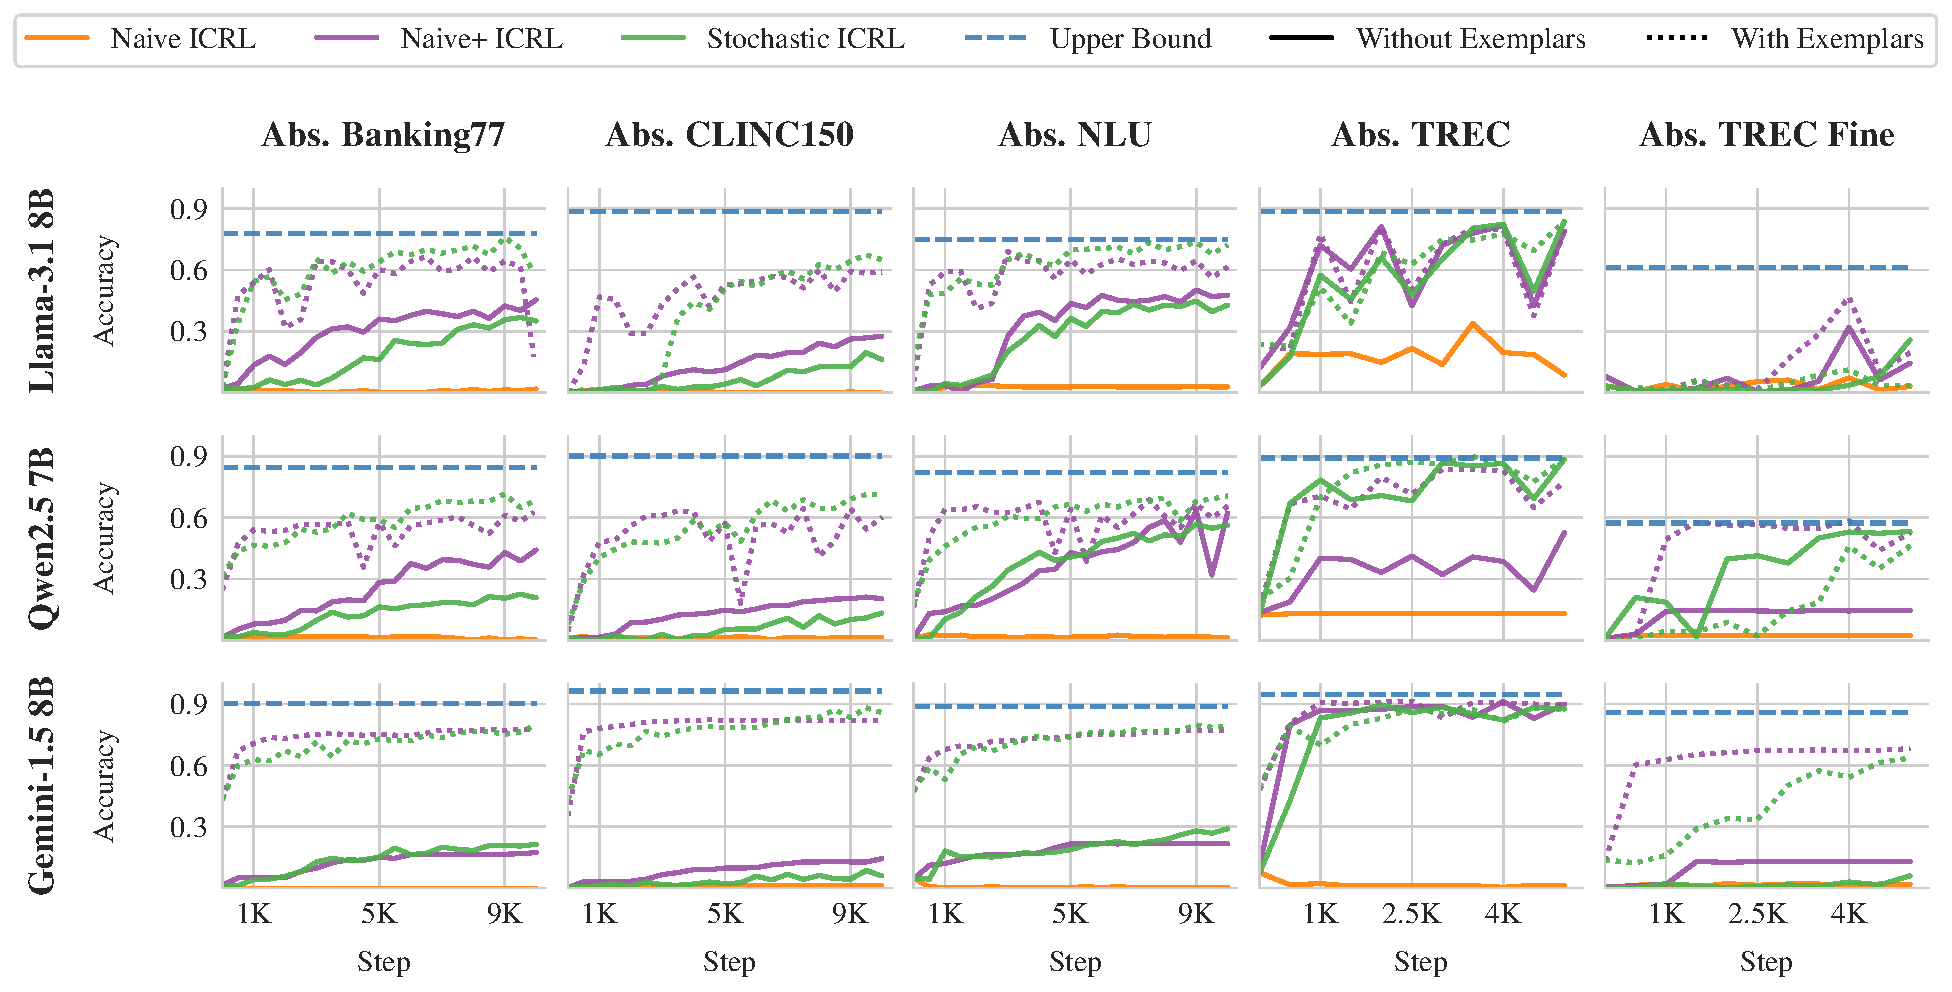
\includegraphics[width=0.99\textwidth]{figures/unsemantic_tasks/all_results.pdf}
    \caption{\textbf{ICRL with Abstract Labels.} We evaluate whether LLMs can learn tasks whose labels carry no semantic meaning by mapping each label to \texttt{label\_{\{number\}}}. Even without initial exemplar demonstrations, \qwen and \llama show increasing performance over time. \gemini similarly excels when given an initial mapping, but struggles in a purely exploratory setting. \autoref{tab:abstract_tasks} in \aautoref{sec:appendix:results} details start and end accuracies.} \label{fig:abstract_tasks}
\vspace{-15pt}
\end{figure*}












\begin{figure*}[t!]
    \centering
    \begin{subfigure}[b]{0.99\textwidth}
        \centering
        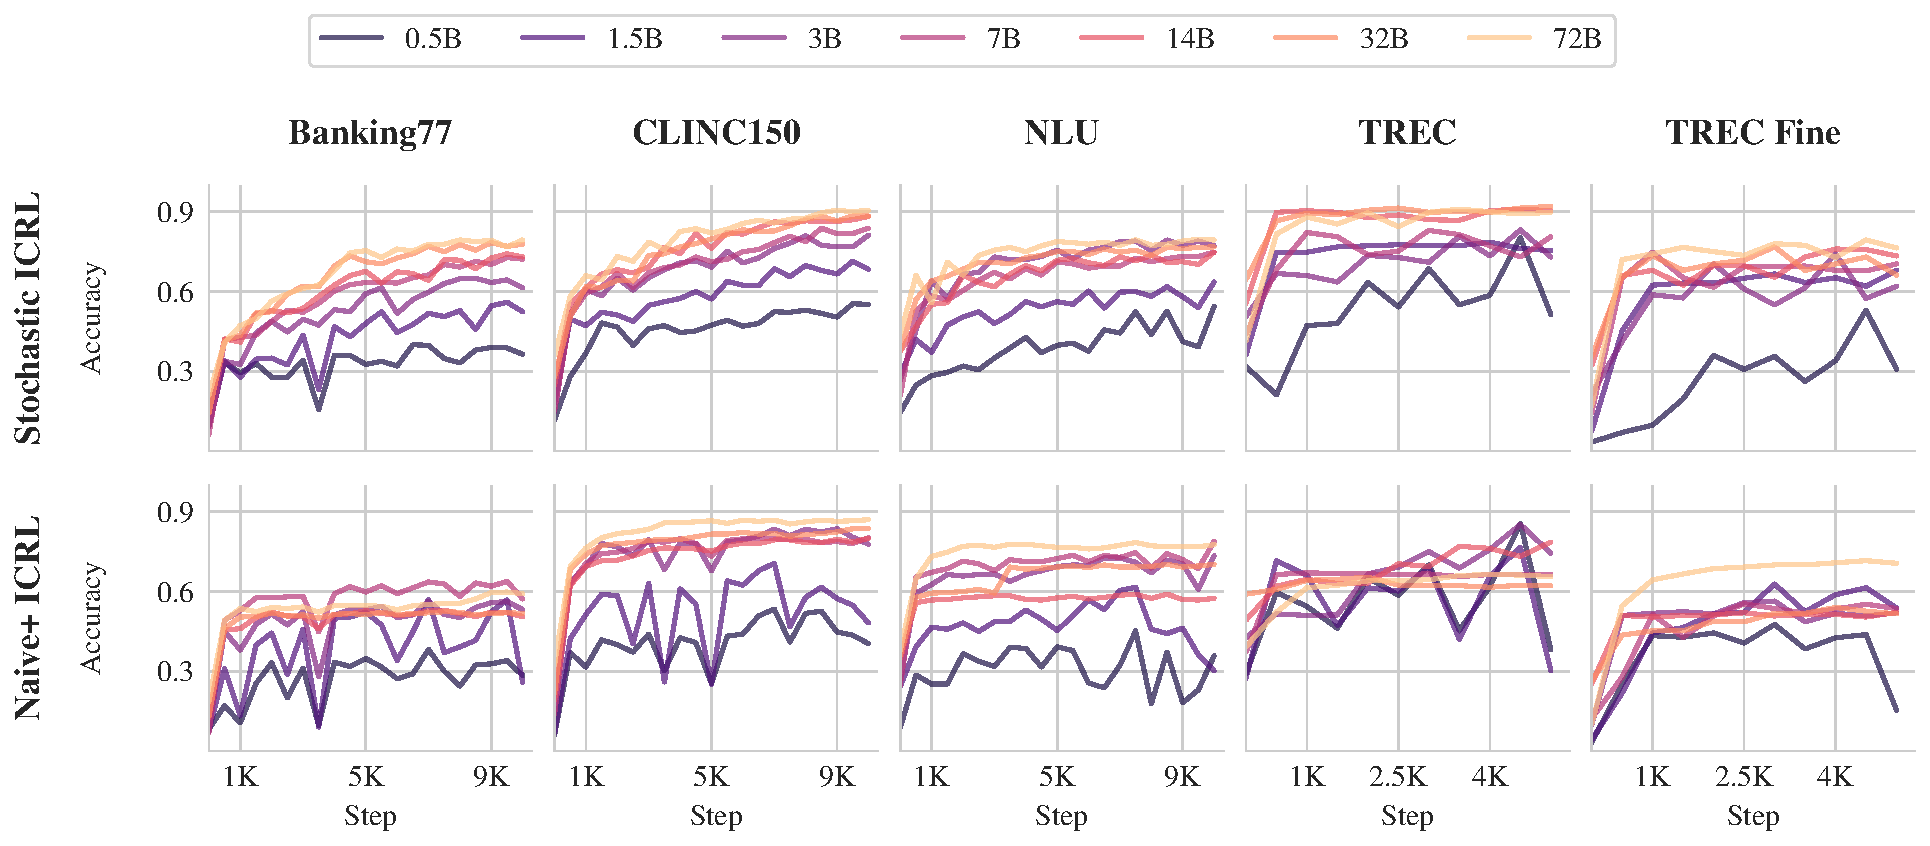
\includegraphics[width=\textwidth]{figures/main_results/qwen_scaling_compact.pdf}
        \caption{\textbf{ICRL Scaling Trends.} We evaluate \qwen models from 500M to 70B parameters using both \naiveplusshort and \expshort. 
        Performance improves substantially over zero-shot accuracy for all sizes, but smaller models plateau at lower accuracies, indicating that ICRL performance correlates positively with model size. \autoref{tab:scaling_compact} in \aautoref{sec:appendix:results} details start and end accuracies.}
        \label{fig:scaling_compact}
    \end{subfigure}
    
    \vspace{1em}
    
    \begin{subfigure}[b]{0.99\textwidth}
        \centering
        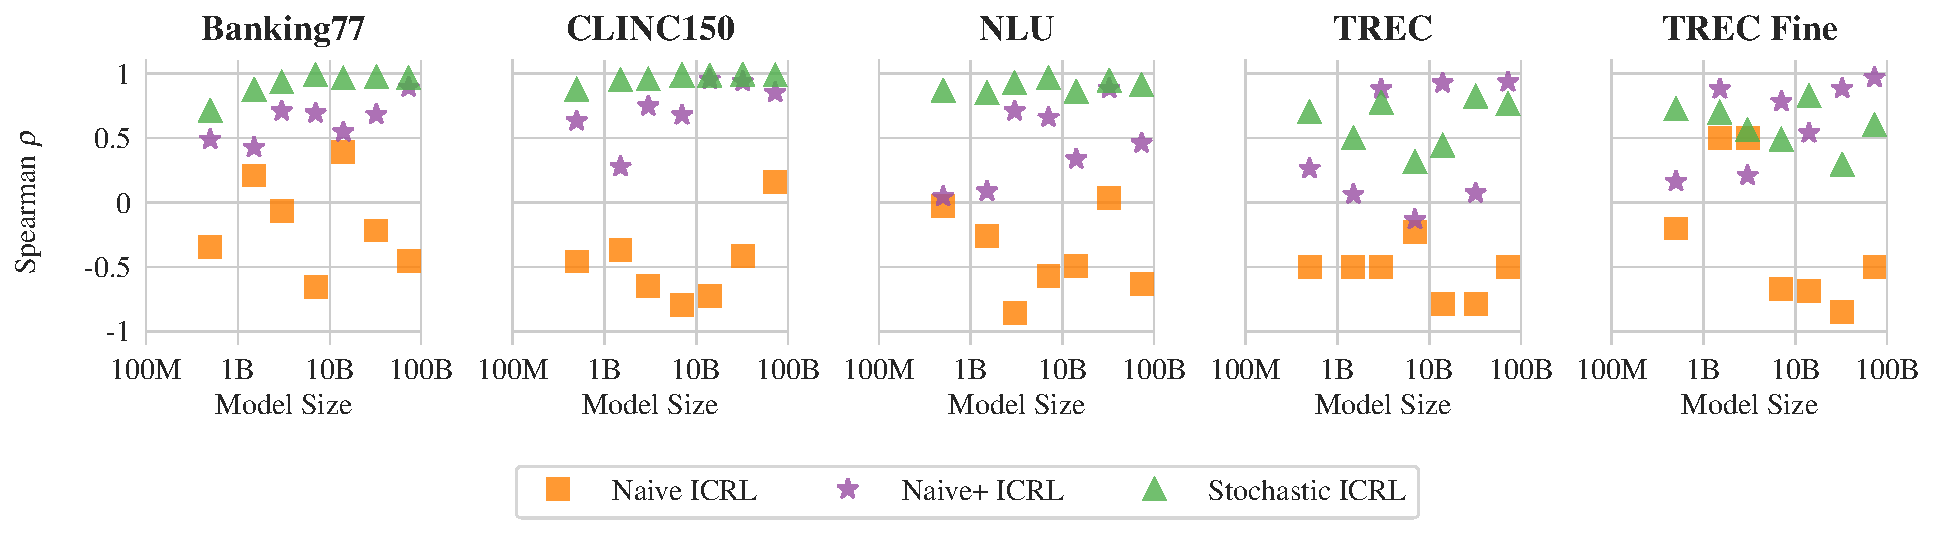
\includegraphics[width=\textwidth]{figures/main_results/qwen_scaling_stability.pdf}
        \caption{\textbf{Stability of \naiveplusshort and \explorative.} We measure stability by computing Spearman’s rank correlation between accuracy and time step. 
        Except for \trec and \trecfine (which give inconclusive results), \expshort exhibits more stable learning on \banking, \clinic, and \nlu. 
        Larger models also show higher stability, mirroring trends in (a). \autoref{tab:qwen_stability} in \aautoref{sec:appendix:results} details $\rho$ values.}
        \label{fig:qwen_stability}
    \end{subfigure}
    \caption{\textbf{Comparison of \qwen models (500M--72B).} We analyze scaling accuracy gains (a) and stability differences (b).}
    \label{fig:combined_scaling}
\vspace{-10pt}
\end{figure*}









\paragraph{Label Semantics Contribute, but ICRL Occurs Without It }
Previous supervised ICL work has shown that LLMs can learn tasks whose labels have no semantic meaning~\citep{pan-etal-2023-context, li2024languagemodelslearncontext}, that is, tasks with \textit{abstract labels}. 
This poses a harder challenge than with labels with semantic meaning, because cannot rely on pre-trained input-output associations. 
We experiment with removing all semantic information from the label space, by mapping each original label to a format \texttt{label\_{\{number\}}}.\footnote{We assign each unique label a random integer from \texttt{1000} onward, up to the total number of labels in a given task.} This ensures that the labels themselves carry no meaningful information that might help the model.
We evaluate two scenarios. In the first and more challenging setup (\textit{Without Exemplars}), we provide no prior demonstrations of correct input-output mappings, thus adhering closely to the ICRL protocol. In the second setup (\textit{With Exemplars}), we give exactly one correct demonstration per label at the start of the prompt (i.e., before past episodes). 



\autoref{fig:abstract_tasks} summarizes our findings on \llama 8B, \qwen{2.5} 7B, and \gemini 1.5 Flash 8B. 
To contextualize the results, we include upper bound results from standard supervised ICL with as many gold demonstrations (with abstract labels) as the context can handle, which generally succeeds across tasks (except for a lower performance on \trecfine). 
With just one exemplar per label, ICRL nearly reaches the upper bound for all tasks and models. We also stress that just including one gold demonstration per label is not always enough to reach good performance, and the online process is still important: for example, \llama with exemplars, when tested on \clinic with \expshort, reaches non-negligible accuracies only after 3k steps.  In the absence of any exemplars, the ICRL process still manages to build informative contexts, though overall accuracy is not surprisingly lower. 
For instance, \qwen and \llama achieve higher than 45\% accuracy on \nlu and \trec with both \naiveplusshort and \expshort, indicating that the models learn and refine their output mappings over time. In contrast, \gemini excels when the correct mapping is provided but struggles significantly in a purely exploratory setting.

Given the domain effect observed with semantic labels, and the relatively low, even if significant results observed with abstract labels, the question arises if this learning is due to a domain effect. 
For example, \llama on \clinic improves from 0.8$\rightarrow$27.6\% during learning with \naiveplusshort, a significant, but modest improvement. 
We ran additional experiments to study the presence of learning with abstract labels, but without reward signals (i.e., to measure the domain effect). We see no improvement over zero-shot performance, confirming the reward signal is what drives learning.\footnote{Because these experiments showed no learning effect at all, we are omitting them from our figures.} 





\paragraph{Bigger Models Are Better at ICRL}

We evaluate  \qwen Instruct models ranging from 500M to 72B parameters using both \naiveplusshort and \expshort to characterize the scaling trends of ICRL. 
\autoref{fig:scaling_compact} shows the results. 
For all model sizes, performance improves substantially over zero-shot accuracy (measured at the first time step). 
However, smaller models tend to plateau at lower accuracies compared to larger models, indicating that ICRL benefits from model scale, similar to other LLM behaviors. 

\paragraph{\expshort is More Stable Than \naiveplusshort}

An important differentiating factor between \expshort and \naiveplusshort is stability. 
The results so far (Figures \ref{fig:main_results}, \ref{fig:abstract_tasks}, and \ref{fig:scaling_compact}) often show sudden, even if temporary dips in performance with \naiveplusshort. 
This instability is undesirable, because it means the performance of the model in interactions (i.e., with users) temporarily deteriorates significantly. 
In contrast, \expshort's learning trends are more stable. 

We quantify stability as Spearman’s rank correlation ($\rho$) between accuracy and time step.\footnote{A perfect positive correlation ($\rho = 1$) indicates strictly increasing accuracy over time, whereas $\rho = -1$ means performance strictly decreases.}  
\autoref{fig:qwen_stability} shows the relation between stability and model sizes for all \qwen models for the three methods. 
Except for \trec and \trecfine, which give inconclusive results, \expshort exhibits more stable learning than \naiveplusshort on \banking, \clinic, and \nlu across all model scales.  
As expected, in general, larger models show higher stability, mirroring the trends in \autoref{fig:scaling_compact}. 
We hypothesize that \expshort is less sensitive to short-term fluctuations, as it relies on a smaller but more diverse set of episodes at each step.

